%!TEX root=report.tex
\subsection{Splines}
Using nine knots with a year in between and letting the sine and cosine functions enter at each knot, one can allow for different seasons. The columns in $X$ can be visualized as in Figure \ref{fig:splines-x-columns}.
\begin{figure}[H]
	\centering
	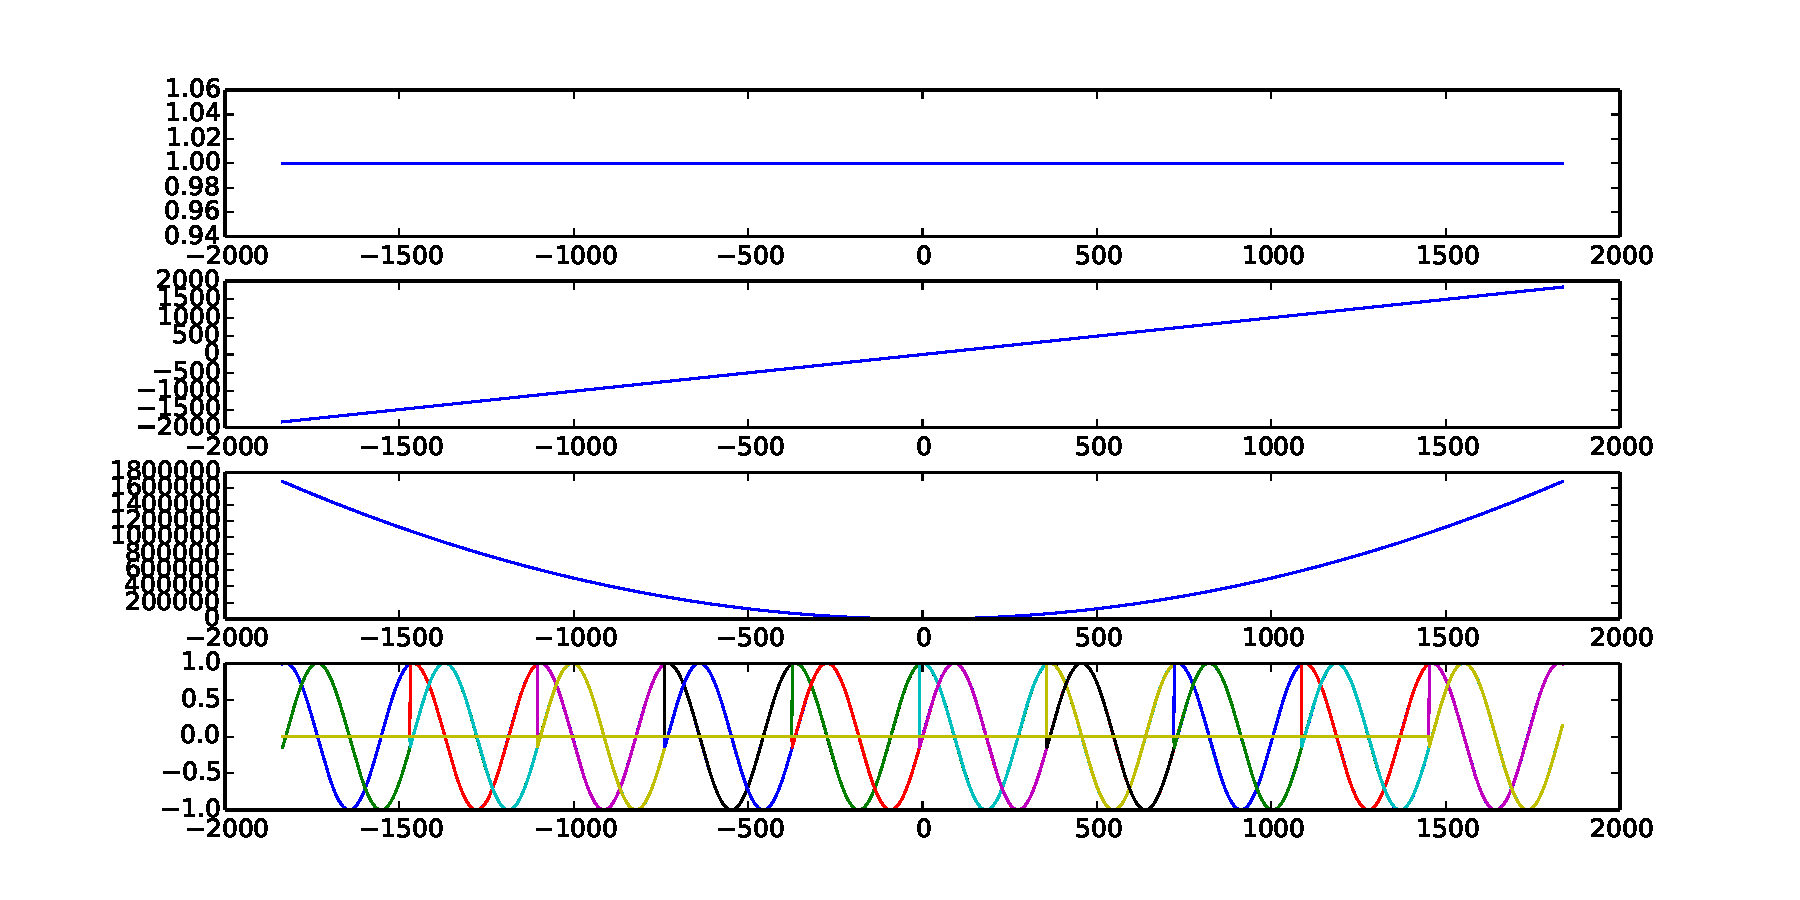
\includegraphics[width=\textwidth]{figures/splines-x-columns}
	\caption{Constant, trend and acceleration in the three uppermost plots. Sine and cosine hinge functions in the bottom plot.}
	\label{fig:splines-x-columns}
\end{figure}

A RMSE diagnostic shows that the residuals are indeed smaller (max standard OLS was 0.135).

\begin{figure}[H]
	\centering
	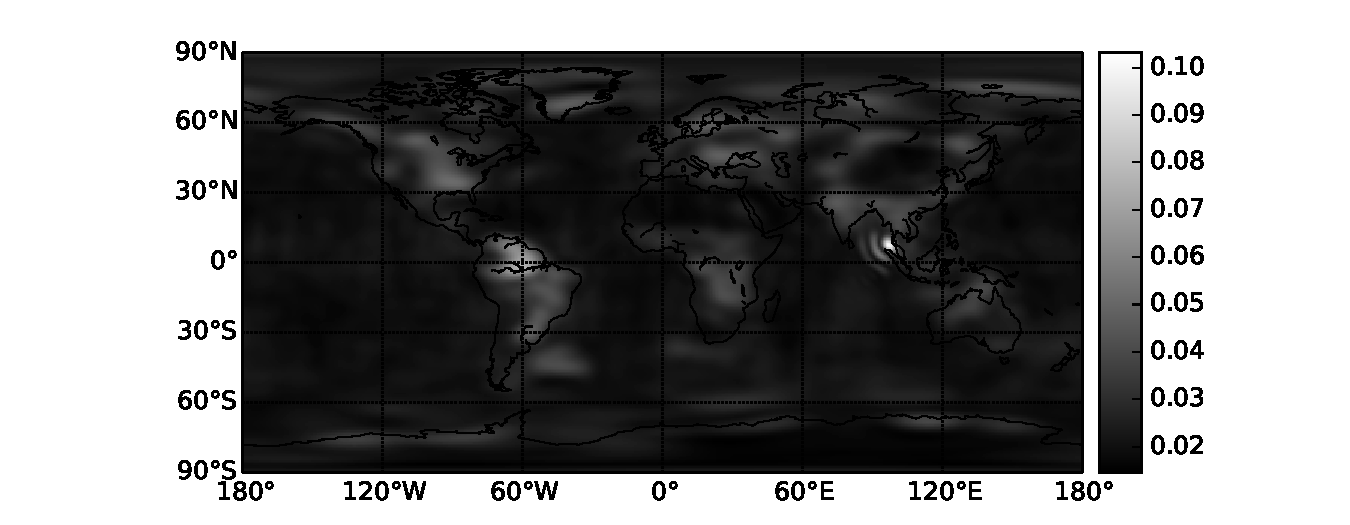
\includegraphics[width=\textwidth]{figures/splines-rmse}
	\caption{RMSE for each position using basis expansion.}
	\label{fig:splines-rmse}
\end{figure}

Looking at the west coast of Greenland now using a basis expansion, the overall fit (Figure \ref{fig:splines-selected-0-fit}) looks improved. For some reason 2009 still causes some issues, which is partially seen in the residuals (Figure \label{fig:splines-selected-0-residual}). Another thing to notices is that the curves are a lot more smooth, but this is simply because only the first 3 frequencies (year, half year and quarter year) was used. This was to prevent the degrees of freedom to drop dramatically, dude to the otherwise huge amount of parameters.
\begin{figure}[H]
	\centering
	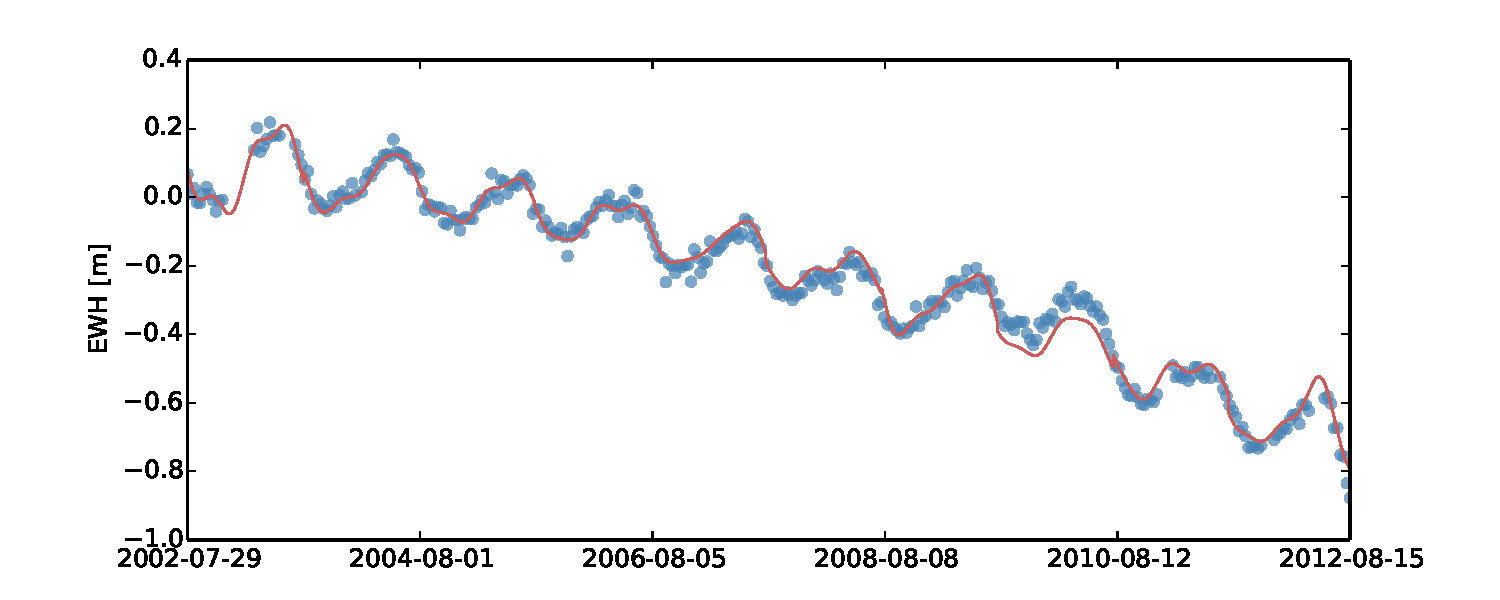
\includegraphics[width=\textwidth]{figures/splines-selected-0-fit}
	\caption{Measurements are blue, the OLS fit is red.}
	\label{fig:splines-selected-0-fit}
\end{figure}

\begin{figure}[H]
	\centering
	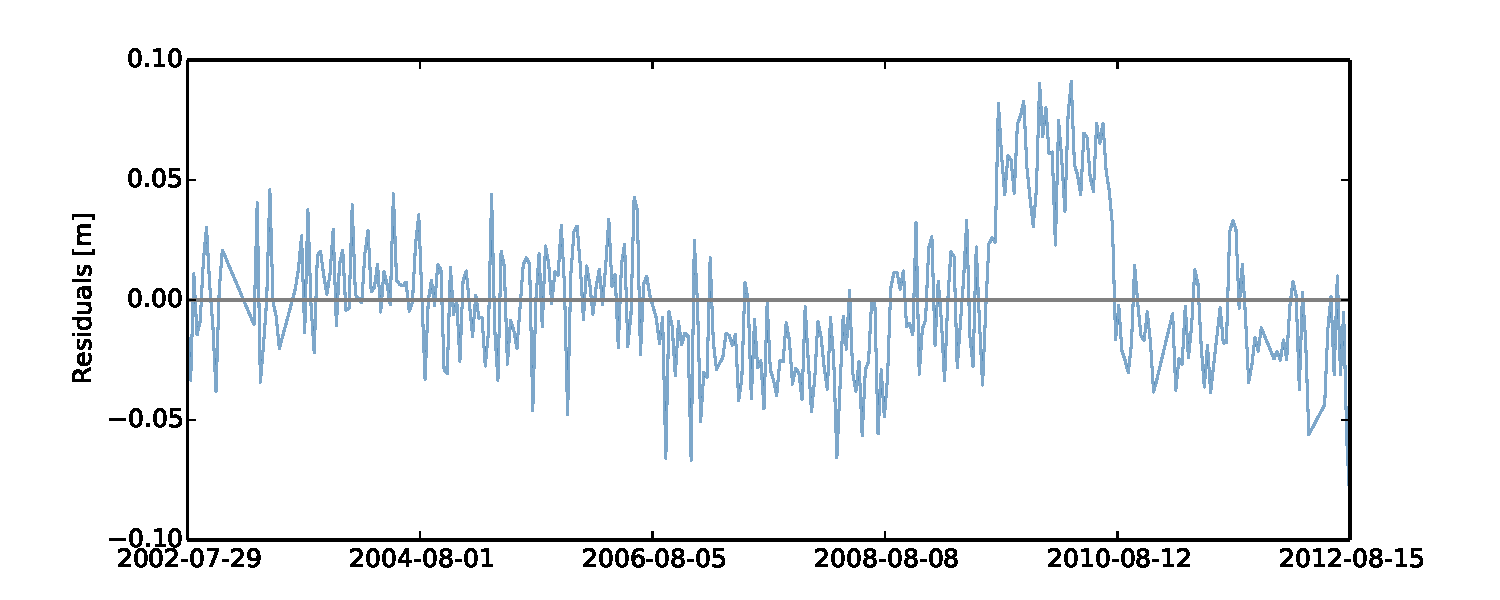
\includegraphics[width=\textwidth]{figures/splines-selected-0-residual}
	\caption{The OLS residuals are blue.}
	\label{fig:splines-selected-0-residual}
\end{figure}

Unfortunately for the south pole, the resulting fits do display some cusps and overfitting behavior. This is particularly seen at 2006 and 2008. Here the residuals haven't improved much, however interestingly enough there now appear to be a two year seasonal trend, between 2003 and 2007. 

\begin{figure}[H]
	\centering
	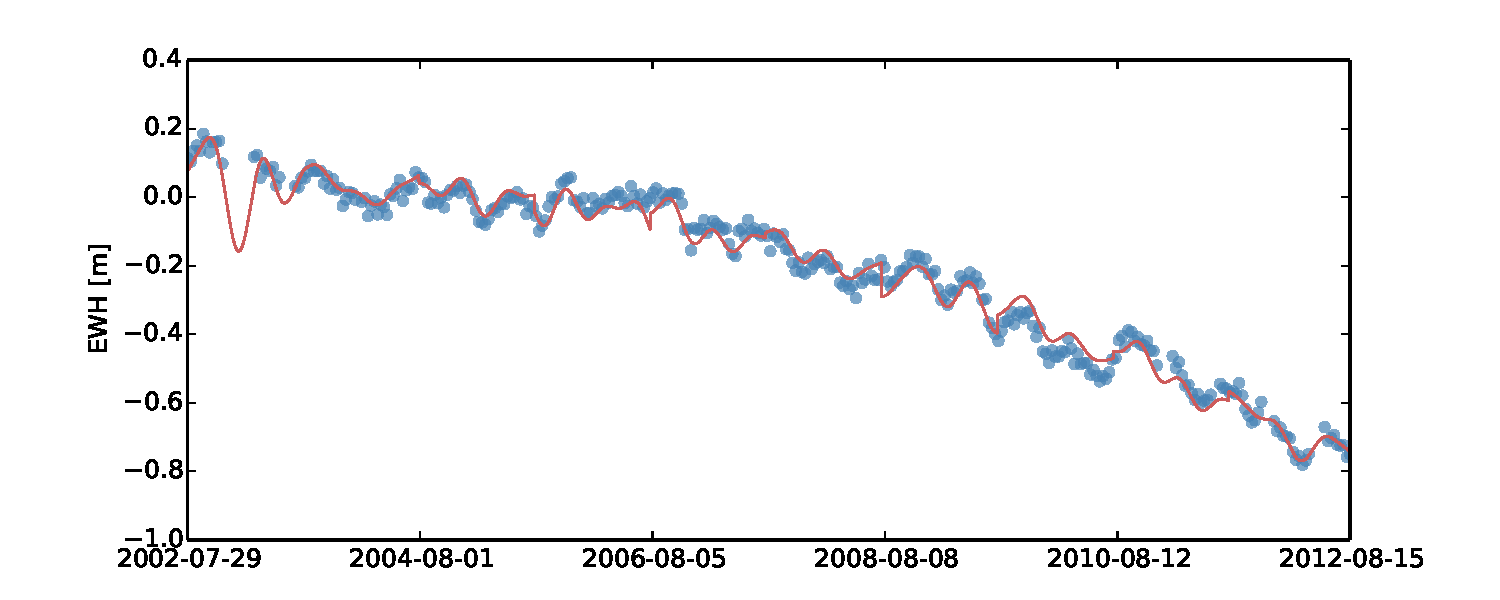
\includegraphics[width=\textwidth]{figures/splines-selected-1-fit}
	\caption{Measurements are blue, the OLS fit is red.}
	\label{fig:splines-selected-1-fit}
\end{figure}

\begin{figure}[H]
	\centering
	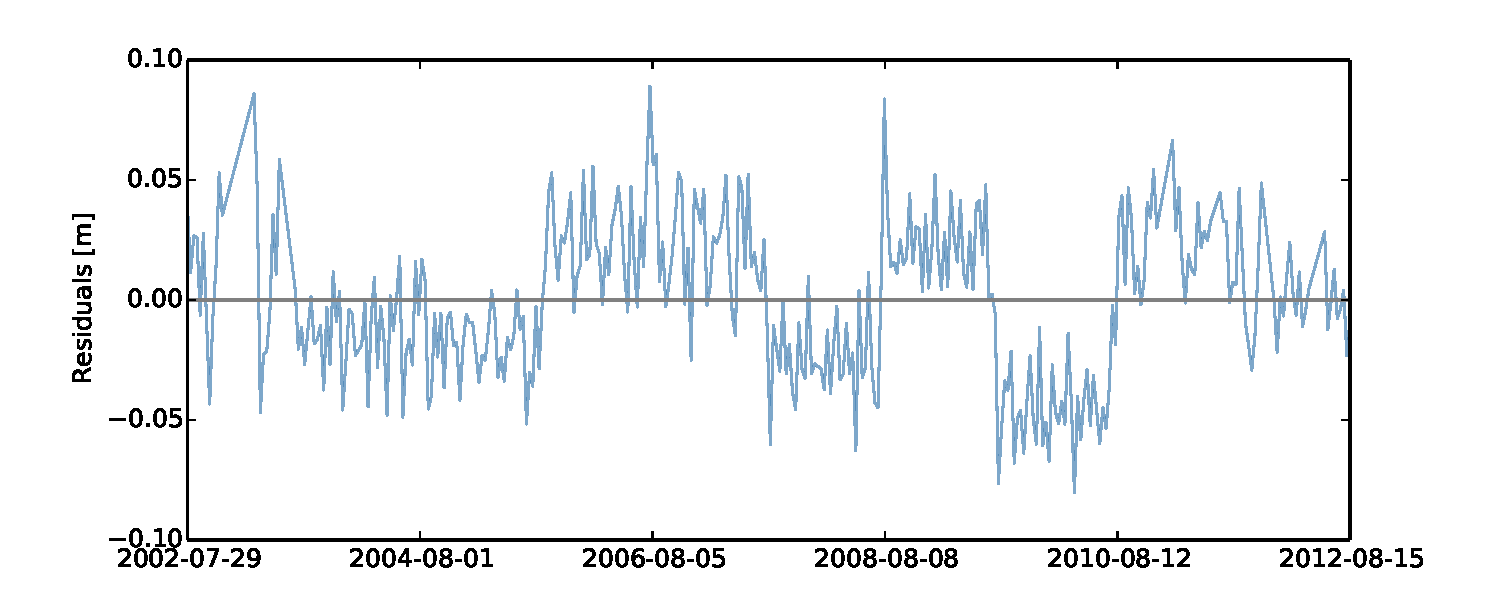
\includegraphics[width=\textwidth]{figures/splines-selected-1-residual}
	\caption{The OLS residuals are blue.}
	\label{fig:splines-selected-1-residual}
\end{figure}
